% base_connaissance.tex

\begin{frame}
	\frametitle{Base de connaissance}
	\begin{figure}[H]
	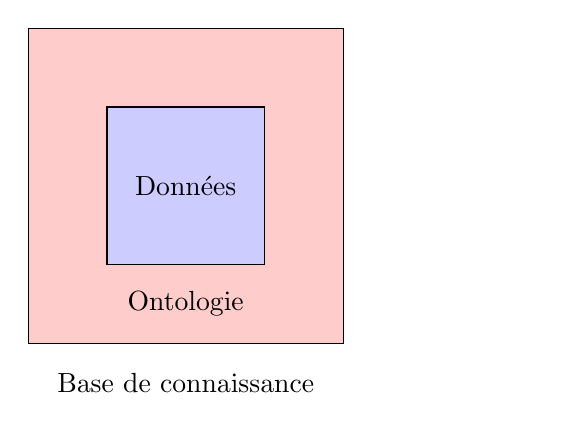
\begin{tikzpicture}[auto,node distance=1.5cm,inner sep=1mm]
%		\node [rectangle,draw,minimum size=6cm] (cr) [] {};
		\node [rectangle,draw,fill=red!20,minimum size=4cm] (or) [] {};
		\node [rectangle,draw,fill=blue!20,minimum size=2cm] (fr) [] {};
		\node [] (c) at(0,-2.5) {Base de connaissance};
		\node [] (o) at(0,-1.5) {Ontologie};
		\node [] (f) [] {Données};
		\node [fill=white!0,rectangle,minimum size=10mm] (sp) at (4,0) {};
	\end{tikzpicture}
	\end{figure}
	\hspace{10mm}
\end{frame}

\begin{frame}
	\frametitle{Base de connaissance}
	\begin{figure}[H]
	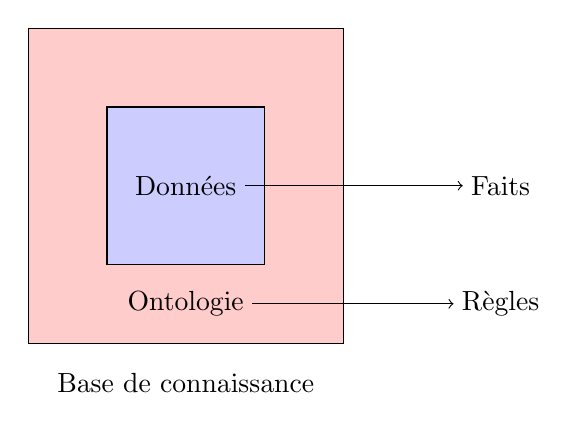
\begin{tikzpicture}[auto,node distance=1.5cm,inner sep=1mm]
%		\node [rectangle,draw,minimum size=6cm] (cr) [] {};
		\node [rectangle,draw,fill=red!20,minimum size=4cm] (or) [] {};
		\node [rectangle,draw,fill=blue!20,minimum size=2cm] (fr) [] {};
		\node [] (c) at(0,-2.5) {Base de connaissance};
		\node [] (o) at(0,-1.5) {Ontologie};
		\node [] (f) [] {Données};
		\node [] (facts) at (4,0) {Faits} 
			edge [<-] (f);
		\node [] (rules) at (4,-1.5) {Règles}
			edge [<-] (o);
	\end{tikzpicture}
	\end{figure}
\end{frame}

\begin{frame}[t]
	\frametitle{Exemples}
	\begin{exampleblock}{Exemple de requête sur les données uniquement}
		Données :
		\begin{itemize}
			\item "{\em Jean} est un des {\em parents} de {\em Tom}"
			\item "{\em Jean} est un {\em homme}"
		\end{itemize}
		Requête : "Jean est-il le père de Tom ?"\\
		Réponse : NON.
	\end{exampleblock}
\end{frame}

\begin{frame}[t]
	\frametitle{Exemples}
	\begin{exampleblock}{Exemple de requête sur les données uniquement}
		Données :
		\begin{itemize}
			\item "{\em Jean} est un des {\em parents} de {\em Tom}"
			\item "{\em Jean} est un {\em homme}"
		\end{itemize}
		Requête : "Jean est-il le père de Tom ?"\\
		Réponse : NON.
	\end{exampleblock}
	\begin{exampleblock}{Et en tenant compte d'une ontologie}
		Ontologie :
		\begin{itemize}
			\item "{\bf Si} un {\em homme} est le {\em parent} de {\em quelqu'un}, {\bf
			alors} {\em il} est son {\em père}." 
		\end{itemize}
		Requête : "Jean est-il le père de Tom ?"\\
		Réponse : OUI.
	\end{exampleblock}
\end{frame}
% on a appliqué la règle
% c'était facile mais en vrai ça l'est pas :
\begin{frame}[t]
	\frametitle{Réponse à une requête}
	\begin{itemize}
		\item Difficulté dépendant de l'ontologie
%		\item  en "général" facile car que de l'universel
%%%%%%%%%%% dans le sens on est sûr de trouver la réponse en temps fini
		\item Possibilité de créer de nouveaux individus
		\item Problème non décidable de manière générale
		\item Nécessaire de déterminer des classes de règles
	\end{itemize}
	\begin{exampleblock}{Exemple}
		Donnée :
		\begin{itemize}
			\item "{\em Jean} est un {\em homme}."
		\end{itemize}
		Ontologie :
		\begin{itemize}
			\item "{\em Tout homme} a un {\em père}."
		\end{itemize}
		Déductions :
		\begin{itemize}
			\item "Jean a un père"
			\item "Celui-ci a un père"
			\item "Ce-dernier a également un père"
			\item ...
		\end{itemize}
	\end{exampleblock}
\end{frame}

